\begin{figure}[t]
  \centering
  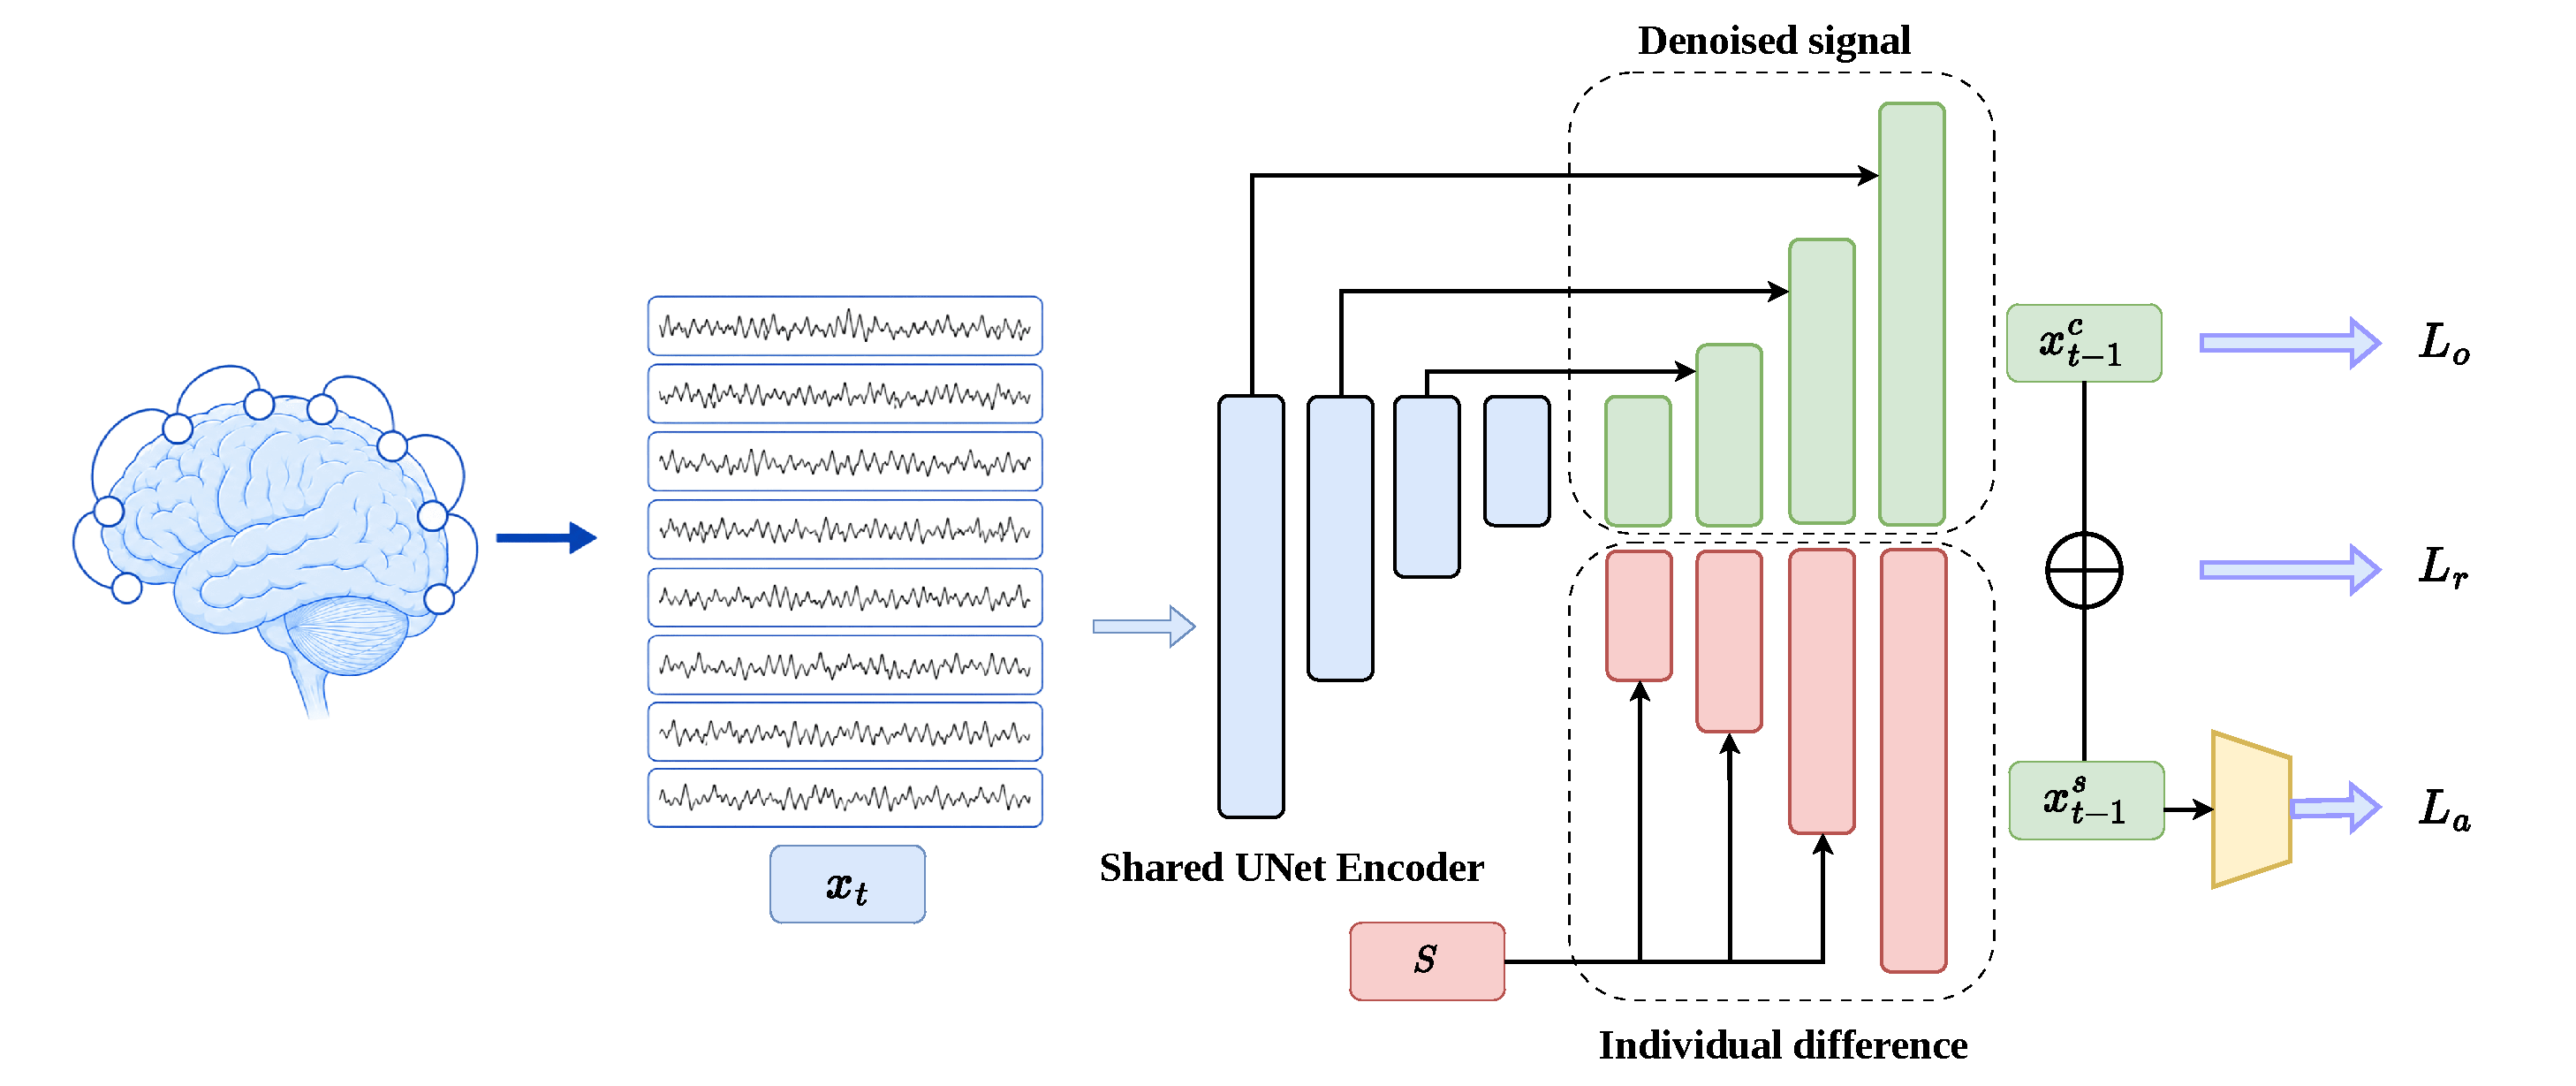
\includegraphics[width=\linewidth]{figures/architecture}
  \caption{Overall architecture of \saddpm{}. Multi-channel EEG is treated as the
  noisy diffusion state $\mathbf{x}_t$ and passed through a \emph{shared
  1D-Conv U-Net encoder}. Two decoder branches share this encoder: a
  \emph{denoised-signal} (content) decoder and an \emph{individual-difference}
  decoder that is conditioned on the subject embedding $\mathbf{e}(s)$. Consistent
  with Eqs.~\eqref{eq:combined_epsilon}--\eqref{eq:reverse_mean_combined}, the two
  branches predict \emph{noise components}: the content noise
  $\boldsymbol{\epsilon}^{c}_{\theta}(\mathbf{x}_t,t)$ and the subject-conditioned
  residual noise $\boldsymbol{\epsilon}^{s}_{\phi}(\mathbf{x}_t,t,\mathbf{e}(s))$.
  Their sum ($\oplus$) is the combined noise estimate
  $\widehat{\boldsymbol{\epsilon}}_{\theta,\phi}$
  (Eq.~\eqref{eq:combined_epsilon}), which determines the reverse-step estimate
  $\mathbf{x}_{t-1}$ through the DDPM reverse mean
  (Eq.~\eqref{eq:reverse_mean_combined}); the branch boxes are labeled with the
  equivalent reverse-step signal contributions
  $\mathbf{x}_{t-1}^{c},\mathbf{x}_{t-1}^{s}$, which are affine images of
  $\boldsymbol{\epsilon}^{c}_{\theta},\boldsymbol{\epsilon}^{s}_{\phi}$ under that
  same map, so the figure and the noise-prediction equations describe the same two
  branches. A classifier head reads the subject branch. Training uses three losses
  (Section~\ref{sec:method_loss}): the orthogonality loss $\mathcal{L}_o$ on the
  content branch, the reverse (reconstruction) loss $\mathcal{L}_r$ on the combined
  estimate, and the angular-margin subject-discrimination loss $\mathcal{L}_a$ on
  the classifier.}
  \label{fig:architecture}
  \Description{A left-to-right schematic. On the left, a head/brain icon produces
  multi-channel EEG shown as stacked time series, denoted as the noisy diffusion
  state x_t. This enters a shared U-Net encoder (a stack of blocks that shrink in
  size). From the encoder, two parallel decoder stacks expand back up: an upper
  ``denoised signal'' (content) branch predicting the content noise component
  epsilon^c_theta, and a lower ``individual difference'' branch, conditioned on a
  subject embedding e(s), predicting the subject-conditioned residual noise
  component epsilon^s_phi. A classifier reads the subject-branch representation.
  The two noise components are summed into the combined noise estimate, which via
  the DDPM reverse mean yields the reverse-step signal x_{t-1}; the branch boxes
  are labeled with the equivalent signal contributions x_{t-1}^c and x_{t-1}^s.
  Three losses are attached: an orthogonality loss on the content branch, a
  reconstruction loss on the combined estimate, and a subject-discrimination loss
  on the classifier.}
\end{figure}
